\documentclass[5pt,a4paper,twocolumn]{article}
\usepackage{geometry}
\usepackage{xeCJK}
\usepackage{indentfirst}
\usepackage{graphicx}
\usepackage{wrapfig}
\usepackage{fontspec}
\usepackage{float}
\usepackage{setspace}
\usepackage{titlesec}
\geometry{left=0.5cm,right=0.5cm,top=0.5cm,bottom=0.5cm} 
\setlength{\abovecaptionskip}{0.1cm}
\setlength{\belowcaptionskip}{0.1cm}
\setCJKmainfont{Microsoft YaHei}
\setmainfont{Microsoft Sans Serif}
\setlength{\parindent}{1em}
\renewcommand\figurename{图}
\title{REVIEW}
\author{马玉坤}
\date{}
\begin{document}
\subsubsection*{计算机基础}

\begin{center}
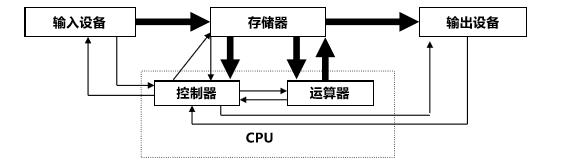
\includegraphics[height=1in]{computer_io.jpg}
\end{center}

\subsubsection*{关键字}
['and', 'as', 'assert', 'break', 'class', 'continue', 'def', 'del', 'elif', 'else', 'except', 'exec', 'finally', 'for', 'from', 'global', 'if', 'import', 'in', 'is', 'lambda', 'not', 'or', 'pass', 'print', 'raise', 'return', 'try', 'while', 'with', 'yield']

\subsubsection*{基本对象类型}
字符串 (string)

整数(integer) 八进制($025$) 十六进制($0x15$)

浮点数(float)

布尔数(boolean)

复数(complex)$3+0.5j$

\subsubsection*{运算符}
运算符优先级从低到高:
\begin{table}[!hbp]
\begin{tabular}{ c c }
lambda & Lambda表达式\\
\hline
or & 布尔“或”\\
\hline
and & 布尔“与”\\
\hline
not & 布尔“非”\\
\hline
in,not in & 成员测试\\
\hline
is,is not & 同一性测试\\
\hline
<,<=,>,>=,!=,== & 比较\\
\hline
| & 按位或\\
\hline
\^{} & 按位异或\\
\hline
\& & 按位与\\
\hline
<<,>> & 移位\\
\hline
+,- & 加法与减法\\
\hline
*,/,\% & 乘法、除法与取余\\
\hline
+x,-x & 正负号\\
\hline
~x & 按位翻转\\
\hline
** & 指数\\
\hline
x.attribute & 属性参考\\
\hline
x[index] & 下标\\
\hline
x[index:index] & 寻址段\\
\hline
f(arguments...) & 函数调用\\
\hline
(experession,...) & 绑定或元组显示\\
\hline
$[expression,...]$ & 列表显示\\
\hline
{key:datum,...} & 字典显示\\
\hline
'expression,...' & 字符串转换\\
\hline
\end{tabular}
\end{table}

\subsubsection*{函数}
函数中的参数名称为“形参”,调用函数时传递的值为“实参”。

为定义在函数外的全局变量赋值需用global。

只有在形参表末尾的那些参数可以有默认参数值,即不能在声明函数形参的时候,先声明有默认值的形参而后声明没有默认值的形参。

func(a=1,b=2)$\sim$func(**{"a":1,"b":2})$\sim$func(*(1,2))

函数只能有一个返回值,但是该值可以是一组值,如返回一个元组。

\subsubsection*{字符串str}

str.capitalize()
Return a copy of the string with its first character capitalized and the rest lowercased.

str.center(width[, fillchar])
Return centered in a string of length width. Padding is done using the specified fillchar (default is a space).

str.count(sub[, start[, end]])
Return the number of non-overlapping occurrences of substring sub in the range [start, end]. Optional arguments start and end are interpreted as in slice notation.

str.find(sub[, start[, end]])
Return the lowest index in the string where substring sub is found, such that sub is contained in the slice s[start:end]. Optional arguments start and end are interpreted as in slice notation. Return -1 if sub is not found.

str.ljust(width[, fillchar])
Return the string left justified in a string of length width. Padding is done using the specified fillchar (default is a space). The original string is returned if width is less than or equal to len(s).

str.center(width[, fillchar])
Return centered in a string of length width. Padding is done using the specified fillchar (default is a space).


\subsubsection*{字符串格式化}
\begin{table}[!hbp]
\begin{tabular}{ c c }
format\_spec & [[fill]align][sign][\#][0][width][,][.precision][type]\\
\hline
fill & <any character>\\
\hline
align & "<" | ">" | "=" | "\^{}"\\
\hline
sign & "+" | "-" | " "\\
\hline
width & integer\\
\hline
precision & integer\\
\hline
type & "b" | "c" | "d" | "e" | "E" | "f" | "F" |\\
&"g" | "G" | "n" | "o" | "s" | "x" | "X" | "\%"\\
\hline

\end{tabular}
\end{table}

\subsubsection*{列表list([..,..])}

L.append(var)   追加元素

L.insert(index,var) 在index位置插入var

L.pop(var)      返回最后一个元素,并从list中删除之

L.remove(var)   删除第一次出现的该元素

L.count(var)    该元素在列表中出现的个数

L.index(var)    该元素的位置,无则抛异常 

L.extend(list)  追加list,即合并list到L上

L.sort()        排序

L.reverse()     倒序

list 操作符:,+,*,关键字del

a[1:]       片段操作符,用于子list的提取

[1,2]+[3,4] 为[1,2,3,4]。同extend()

[2]*4       为[2,2,2,2]

del L[1]    删除指定下标的元素

del L[1:3]  删除指定下标范围的元素

\subsubsection*{字典dict(\{:,..\})}

D.get(key, 0)       同dict[key],多了个没有则返回缺省值,0。[]没有则抛异常

D.has\_key(key)      有该键返回True,否则False

D.keys()            返回字典键的列表

D.values() 返回字典值的列表

D.items() 返回可遍历的字典列表,每一个键值对为一个tuple

D.update(dict2)     增加合并字典

D.popitem()         得到一个pair,并从字典中删除它。已空则抛异常

D.clear()           清空字典,同del dict

D.copy()            拷贝字典

D.cmp(dict1,dict2)  比较字典,(优先级为元素个数、键大小、键值大小),第一个大返回1,小返回-1,一样返回0

\subsubsection*{集合set,frozenset(set([..], frozenset([..]))}

isdisjoint(other)
Return True if the set has no elements in common with other. Sets are disjoint if and only if their intersection is the empty set.

issubset(other)
set <= other
Test whether every element in the set is in other.

set < other
Test whether the set is a proper subset of other, that is, set <= other and set != other.

issuperset(other)
set >= other
Test whether every element in other is in the set.

set > other
Test whether the set is a proper superset of other, that is, set >= other and set != other.

union(other, ...)
set | other | ...
Return a new set with elements from the set and all others.

intersection(other, ...)
set \& other \& ...
Return a new set with elements common to the set and all others.

difference(other, ...)
set - other - ...
Return a new set with elements in the set that are not in the others.

symmetric\_difference(other)
set \^{} other
Return a new set with elements in either the set or other but not both.

copy()
Return a new set with a shallow copy of s.

Note, the non-operator versions of union(), intersection(), difference(), and symmetric\_difference(), issubset(), and issuperset() methods will accept any iterable as an argument. In contrast, their operator based counterparts require their arguments to be sets. This precludes error-prone constructions like set('abc') \& 'cbs' in favor of the more readable set('abc').intersection('cbs').

update(other, ...)
set |= other | ...
Update the set, adding elements from all others.

intersection\_update(other, ...)
set \&= other \& ...
Update the set, keeping only elements found in it and all others.

difference\_update(other, ...)
set -= other | ...
Update the set, removing elements found in others.

symmetric\_difference\_update(other)
set \^{}= other
Update the set, keeping only elements found in either set, but not in both.

以下方法set支持,frozenset不支持

add(elem)
Add element elem to the set.

remove(elem)
Remove element elem from the set. Raises KeyError if elem is not contained in the set.

discard(elem)
Remove element elem from the set if it is present.

pop()
Remove and return an arbitrary element from the set. Raises KeyError if the set is empty.

\subsubsection*{数据结构性质总结}
\begin{table}[!hbp]
\begin{tabular}{ c c c c c c }
&string & list & tuple & set & dict\\
\hline
Mutable & No & Yes & No & Yes & Yes\\
\hline
Sequential & Yes & Yes & Yes & No & No\\
\hline
Sortable & No & Yes & No & No & No\\
\hline
Slicable & Yes & Yes & Yes & No & No\\
\hline
Index/key type & Int & Int & Int & Immut& Immut\\
\hline
Item/value type & Char & Any & Any & No & Any\\
\hline
Search complexity & O(n) & O(n) & O(n) & O(1) & O(1)\\
\hline
\end{tabular}
\end{table}

\subsubsection*{正则表达式re}

ptn = re.compile(r'..') \#ptn is a Pattern\\
Pattern属性:

pattern: 编译时用的表达式字符串。

flags: 编译时用的匹配模式。数字形式。

groups: 表达式中分组的数量。

groupindex: 以表达式中有别名的组的别名为键、以该组对应的编号为值的字典,没有别名的组不包含在内。

Pattern实例方法[ | re模块方法]:

match(string[, pos[, endpos]]) | re.match(pattern, string[, flags]) 
这个方法将从string的pos下标处起尝试匹配pattern;如果pattern结束时仍可匹配,则返回一个Match对象;如果匹配过程中pattern无法匹配,或者匹配未结束就已到达endpos,则返回None。 
pos和endpos的默认值分别为0和len(string);re.match()无法指定这两个参数,参数flags用于编译pattern时指定匹配模式。 
注意:这个方法并不是完全匹配。当pattern结束时若string还有剩余字符,仍然视为成功。想要完全匹配,可以在表达式末尾加上边界匹配符'$\backslash$\$'。

search(string[, pos[, endpos]]) | re.search(pattern, string[, flags])
这个方法用于查找字符串中可以匹配成功的子串。从string的pos下标处起尝试匹配pattern,如果pattern结束时仍可匹配,则返回一个Match对象;若无法匹配,则将pos加1后重新尝试匹配;直到pos=endpos时仍无法匹配则返回None。 
pos和endpos的默认值分别为0和len(string));re.search()无法指定这两个参数,参数 flags用于编译pattern时指定匹配模式。

split(string[, maxsplit]) | re.split(pattern, string[, maxsplit])
按照能够匹配的子串将string分割后返回列表。maxsplit用于指定最大分割次数,不指定将全部分割。 

findall(string[, pos[, endpos]]) | re.findall(pattern, string[, flags])
搜索string,以列表形式返回全部能匹配的子串。 

finditer(string[, pos[, endpos]]) | re.finditer(pattern, string[, flags])
搜索string,返回一个顺序访问每一个匹配结果(Match对象)的迭代器。 

sub(repl, string[, count]) | re.sub(pattern, repl, string[, count])
使用repl替换string中每一个匹配的子串后返回替换后的字符串。 
当repl是一个字符串时,可以使用$\backslash$id或$\backslash$g<id>、$\backslash$g<name>引用分组,但不能使用编号0。 
当repl是一个方法时,这个方法应当只接受一个参数(Match对象),并返回一个字符串用于替换(返回的字符串中不能再引用分组)。 
count用于指定最多替换次数,不指定时全部替换。 

subn(repl, string[, count]) |re.sub(pattern, repl, string[, count])
返回 (sub(repl, string[, count]), 替换次数)。 

\begin{center}
\begin{figure*}[htbp]
\centering
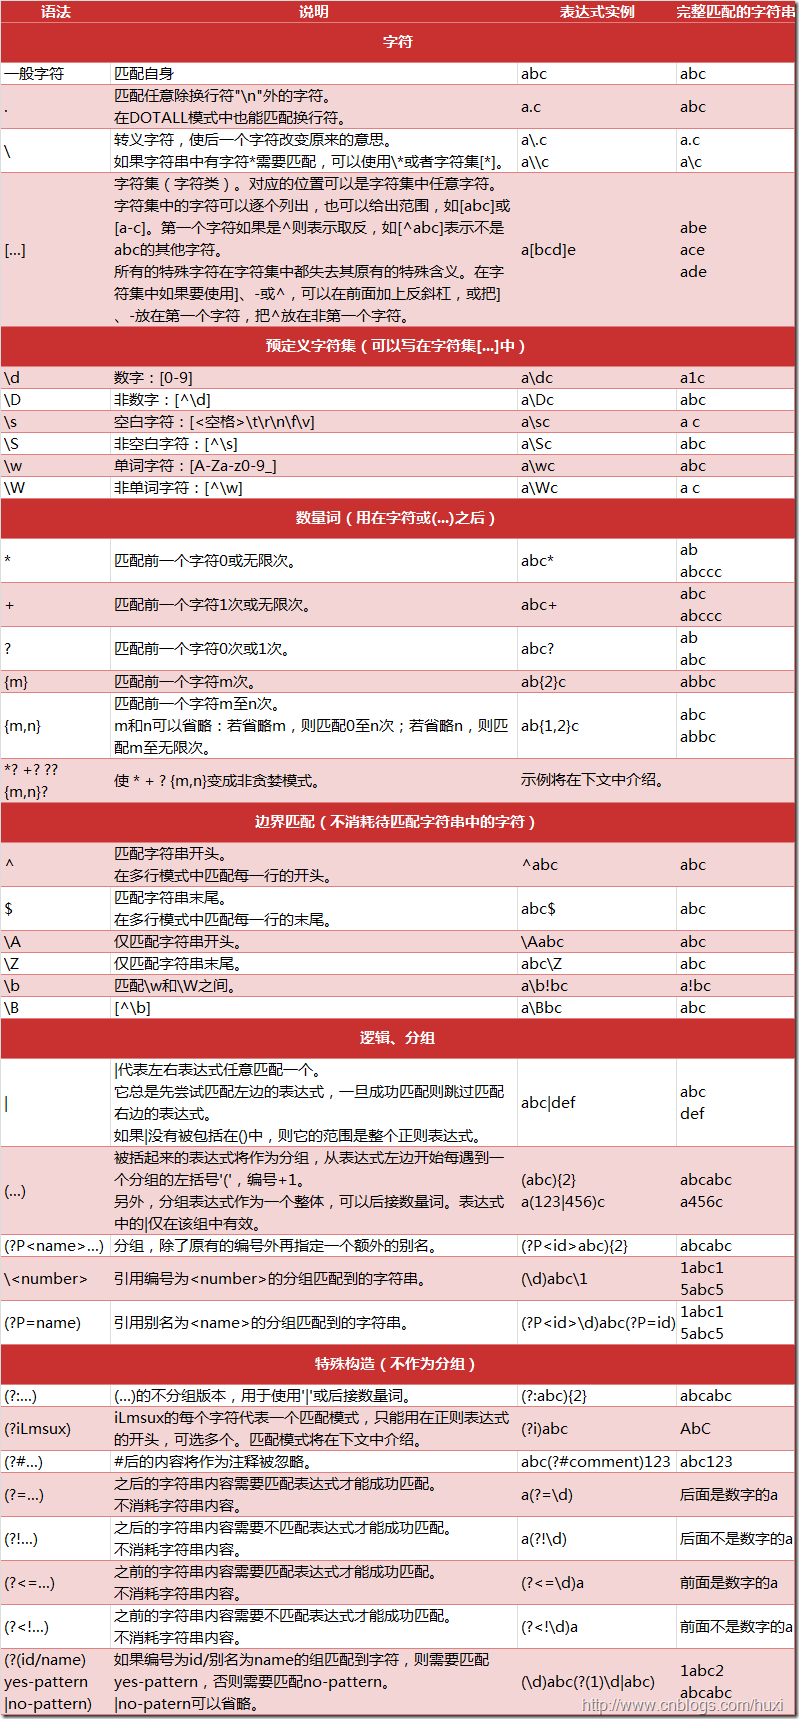
\includegraphics[height=11.5in]{re.jpg}
\end{figure*}
\end{center}

\end{document}
